% Created 2026-07-05 Sun 16:50
% Intended LaTeX compiler: pdflatex
\documentclass[11pt]{article}

\usepackage[utf8]{inputenc}
\usepackage[T1]{fontenc}
\usepackage{graphicx}
\usepackage{longtable}
\usepackage{wrapfig}
\usepackage{rotating}
\usepackage[normalem]{ulem}
\usepackage{amsmath}
\usepackage{amssymb}
\usepackage{capt-of}
\usepackage{hyperref}
\author{SCS}
\date{2026-07-05}
\title{\LaTeX{} export hooks explained}
\hypersetup{
 pdfauthor={SCS},
 pdftitle={\LaTeX{} export hooks explained},
 pdfkeywords={},
 pdfsubject={},
 pdfcreator={},
 pdflang={English}}
\begin{document}

\maketitle
\setcounter{tocdepth}{2}
\tableofcontents

\section*{Overview}
\label{sec:org90e9c2c}

This document explains how Org → \LaTeX{}/PDF export is extended for SCS
checklists and similar documents.  The pieces work together:

\begin{center}
\begin{tabular}{lll}
Component & File & Role\\
\hline
Line-prefix syntax & \texttt{org-tools.el} & \texttt{!} / => shorthands → center / quote blocks\\
Faded letterhead & \texttt{org-tools.el} & Reads Org keywords, builds faded PDF, patches \texttt{.tex}\\
Canon fonts & \texttt{scs-fontspec.tex} & Simoncini body, Adobe Garamond small caps \& headers\\
Org document & e.g. \texttt{packing-list.org} & Keywords, \texttt{\#+LATEX\_HEADER}, body text\\
\end{tabular}
\end{center}

Enable once in your init file:

\begin{verbatim}
(with-eval-after-load 'org
  (require 'org-tools))
\end{verbatim}
\section*{The export pipeline (big picture)}
\label{sec:orgc1f2038}

When you run \texttt{C-c C-e l l} (\LaTeX{} export) or \texttt{C-c C-e l p} (PDF), Org does
not simply “save the buffer as =.tex=”.  Several hooks run in a fixed order.

\begin{center}
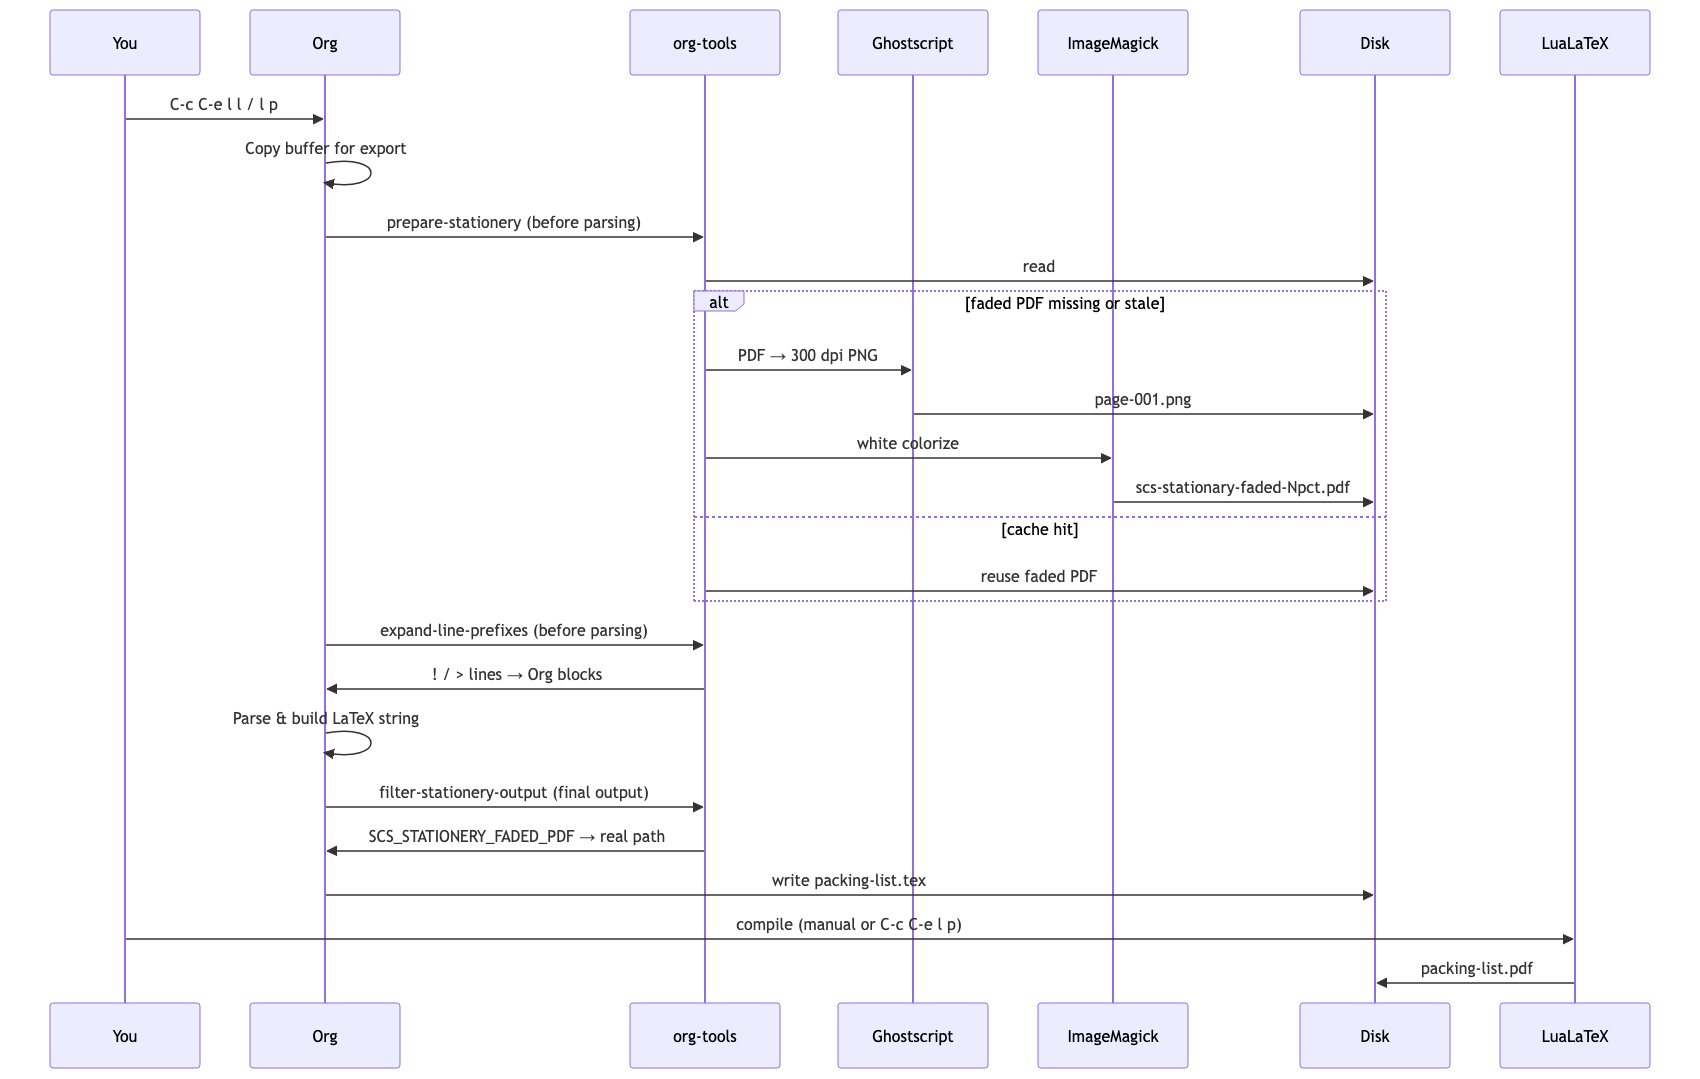
\includegraphics[width=.9\linewidth]{export-pipeline.png}
\label{org625b254}
\end{center}

\textbf{\textbf{Hook registration}} (in \texttt{org-tools.el}):

\begin{center}
\begin{tabular}{lll}
Hook & Function & When\\
\hline
\texttt{org-export-before-parsing-functions} & \texttt{org-tools-prepare-stationery} & Before Org parses export copy\\
\texttt{org-export-before-parsing-functions} & \texttt{org-tools-expand-line-prefixes} & Same phase, after stationery\\
\texttt{org-export-filter-final-output-functions} & \texttt{org-tools-filter-stationery-output} & After full \texttt{.tex} string built\\
\end{tabular}
\end{center}

Stationery runs first (prepends to the hook list after line-prefixes is
registered, so it executes before prefix expansion).
\section*{Line-prefix syntax (! and >)}
\label{sec:orgf68d14d}

Implemented in \texttt{/Users/scs/.config/emacs/lisp/org-tools.el}.

\textbf{\textbf{When it runs:}} \texttt{org-export-before-parsing-functions} →
\texttt{org-tools-expand-line-prefixes}, \textbf{before} Org parses the export buffer.

\textbf{\textbf{Toggle:}} \texttt{M-x org-tools-line-prefixes-mode} / \texttt{M-x org-tools-line-prefixes-status}
\subsection*{Centered lines (\texttt{!})}
\label{sec:orgb53b462}

Consecutive lines starting with \texttt{!} at column 0 become a center block.
Optional style tokens after \texttt{!} apply to that line only.

\begin{verbatim}
!sc large Packing checklist
! (summer — warm season)
\end{verbatim}

\LaTeX{} export (conceptually):

\begin{verbatim}
#+begin_center
@@latex:{\large\textsc{Packing checklist}}@@

(summer — warm season)
#+end_center
\end{verbatim}

\textbf{\textbf{Quote lines (\texttt{>})}}

\begin{verbatim}
> Nothing is compulsory.
> Some items are optional.
\end{verbatim}

becomes:

\begin{verbatim}
#+begin_quote
Nothing is compulsory.

Some items are optional.
#+end_quote
\end{verbatim}

\textbf{\textbf{Style modifiers}} (center lines only, space-separated, case-sensitive):

\begin{center}
\begin{tabular}{ll}
Token & \LaTeX{} effect\\
\hline
\texttt{sc}, \texttt{smallcaps} & \texttt{\textbackslash{}textsc\{...\}} (via \texttt{scs-fontspec.tex})\\
\texttt{tiny} … \texttt{huge}, \texttt{Huge} & \texttt{\textbackslash{}tiny} … \texttt{\textbackslash{}Huge}\\
\texttt{10pt}, \texttt{12.5pt}, etc. & \texttt{\textbackslash{}fontsize\{...\}\{...\}\textbackslash{}selectfont}\\
\end{tabular}
\end{center}

Examples:

\begin{verbatim}
!sc large Main title
!sc footnotesize typeset at tapoban -- 4 july 63 sc
!14pt Subtitle
! Plain centred line
\end{verbatim}

\textbf{\textbf{Rules}}

\begin{itemize}
\item Prefixes start at column 0.
\item A blank line ends the current run.
\item \texttt{!} and => runs do not mix.
\item Lines inside \texttt{\#+begin\_src}, \texttt{\#+begin\_export}, \texttt{\#+begin\_example},
\texttt{\#+begin\_verse} are left untouched.
\end{itemize}

\textbf{\textbf{Footer layout helpers}}

Push a credit line to the bottom of the page:

\begin{verbatim}
#+begin_export latex
\vfill
#+end_export

!sc footnotesize typeset at tapoban on 4 july 63 sc -- sri chinmoy society press
!sc footnotesize [letterhead colours dimmed on purpose]
\end{verbatim}

Use \texttt{\textbackslash{}vspace\{-0.5em\}} after \texttt{\textbackslash{}vfill} if you want the line closer to the
bottom margin.
\section*{Canon fonts (scs-canon)}
\label{sec:orga372174}

\textbf{\textbf{File:}} \texttt{/Users/scs/fonts/scs-canon/scs-fontspec.tex}

All faces live in one directory so fontspec auxiliary fonts (\texttt{SmallCapsFont},
\texttt{BoldFont}, etc.) can share a single \texttt{Path}.  Org files pull it in with:

\begin{verbatim}
#+LATEX_HEADER: \usepackage{microtype}
#+LATEX_HEADER: \input{/Users/scs/fonts/scs-canon/scs-fontspec.tex}
\end{verbatim}

Load \texttt{microtype} \textbf{before} \texttt{scs-fontspec.tex} so \texttt{\textbackslash{}textsc} is reinstalled
correctly after \texttt{microtype} loads.

\textbf{\textbf{Faces configured}}

\begin{center}
\begin{tabular}{lll}
Macro / role & Font file & Notes\\
\hline
Body (\texttt{\textbackslash{}setmainfont}) & \texttt{SimonciniGaramondStd} & Regular, bold, italic\\
\texttt{\textbackslash{}textsc} & \texttt{AGaramondPro-Regular} + \texttt{Letters=SmallCaps} & Simoncini has no smcp glyphs\\
\texttt{\textbackslash{}runheaderfont} & \texttt{AGaramondPro} family & Running headers\\
\texttt{\textbackslash{}runheadertext\{...\}} & wraps \texttt{\textbackslash{}scs@smallcaps} & Safe inside \texttt{\textbackslash{}fancyhead}\\
\end{tabular}
\end{center}

\textbf{\textbf{Why not \texttt{SmallCapsFont=\{AGaramond...\}} alone?}}

\texttt{SmallCapsFont} selects the \textbf{file} for the NFSS \texttt{sc} shape but does not
enable OpenType \texttt{smcp}.  The working approach uses an explicit \texttt{\textbackslash{}fontspec}
call with \texttt{Letters=SmallCaps}:

\begin{verbatim}
\fontspec[Path=..., Letters=SmallCaps, Ligatures=TeX]{AGaramondPro-Regular}{#1}
\end{verbatim}

Important details (learned the hard way):

\begin{center}
\begin{tabular}{lll}
Issue & Cause & Fix\\
\hline
No visible small caps & \texttt{smcp} not enabled & \texttt{Letters=SmallCaps} on \texttt{\textbackslash{}fontspec}\\
Text starting with \texttt{[} vanishes & \texttt{[...]} parsed as fontspec options & Wrap text in \texttt{\{\#1\}} after font name\\
\texttt{-{}-{}} stays as two hyphens & HarfBuzz path skips \TeX{} ligatures & \texttt{Ligatures=TeX} on small-caps \texttt{\textbackslash{}fontspec}\\
Header \texttt{[packing checklist]} broken & \texttt{\#1} in hook macro body & Use \texttt{\#\#1} in \texttt{\textbackslash{}scs@installtextsc}; use \texttt{\textbackslash{}runheadertext}\\
\texttt{\textbackslash{}textsc} broken after \texttt{microtype} & Hook passes args into \texttt{\#1} & \texttt{\textbackslash{}AddToHook\{package/microtype/after\}\{...\}} with \texttt{\#\#1}\\
\end{tabular}
\end{center}

Swap faces by editing the \texttt{\textbackslash{}scs@...} variables at the top of
\texttt{scs-fontspec.tex}.
\section*{Faded letterhead (stationery)}
\label{sec:orgabc7856}

Vector letterhead (\texttt{scs-stationary.pdf}) is PDF/X CMYK.  \LaTeX{}
\texttt{\textbackslash{}includegraphics[opacity=0.5]} had no visible effect.  The working approach
pre-fades via Ghostscript + ImageMagick and includes the rasterised PDF as
background (\texttt{eso-pic}).

\textbf{\textbf{Org file keywords}}

\begin{verbatim}
#+SCS_STATIONERY: /Users/scs/Documents/scs-stationary.pdf
#+SCS_STATIONERY_FADE: 27

#+LATEX_HEADER: \AddToShipoutPictureBG{\AtPageLowerLeft{\includegraphics[width=\paperwidth,height=\paperheight]{SCS_STATIONERY_FADED_PDF}}}
\end{verbatim}

\begin{center}
\begin{tabular}{ll}
Keyword & Meaning\\
\hline
\texttt{\#+SCS\_STATIONERY:} & Source letterhead PDF (default: \texttt{\textasciitilde{}/Documents/scs-stationary.pdf})\\
\texttt{\#+SCS\_STATIONERY\_FADE:} & Percentage of \textbf{original colour kept} (27 = quite faint)\\
\texttt{SCS\_STATIONERY\_FADED\_PDF} & Placeholder in \texttt{\#+LATEX\_HEADER}; replaced in final \texttt{.tex}\\
\end{tabular}
\end{center}

Do \textbf{not} use \texttt{@@SCS\_STATIONERY@@} — Org treats \texttt{@@...@@} as export snippets.

\textbf{\textbf{Cached output path}}

\begin{verbatim}
{source-dir}/{basename}-faded-{N}pct.pdf
\end{verbatim}

Example: \texttt{/Users/scs/Documents/scs-stationary-faded-27pct.pdf}

Changing \texttt{FADE} from 27 to 20 creates a separate cached file;
old percentages remain on disk.

\textbf{\textbf{Fade math}}

\begin{verbatim}
ImageMagick colorize% = 100 − FADE%

FADE 27  →  colorize 73% white  (27% colour remains)
FADE 50  →  colorize 50% white
\end{verbatim}
\section*{Step 2 behind the scenes (raster fade)}
\label{sec:org38715cc}

When \texttt{org-tools-prepare-stationery} runs:

\begin{enumerate}
\item \textbf{Read keywords} from the export buffer (first 32 KiB), via regex on
\texttt{\#+SCS\_STATIONERY:} and \texttt{\#+SCS\_STATIONERY\_FADE:}.
\item \textbf{Compute paths} — source PDF and faded output \texttt{...-faded-Npct.pdf}.
\item \textbf{Skip or rebuild} — rebuild only if faded file missing or older than source.
\item \textbf{Run three external commands} in a temp directory (\texttt{call-process}, not a
shell script on disk):
\end{enumerate}

\begin{center}
\begin{tabular}{llll}
Step & Program & Arguments (conceptually) & Result\\
\hline
A & \texttt{gs} & \texttt{png16m}, \texttt{-r300}, source PDF & \texttt{page-001.png}\\
B & \texttt{magick} & white background, \texttt{-colorize N\%} & \texttt{faded.png}\\
C & \texttt{magick} & 300 dpi, zip compress & \texttt{scs-stationary-faded-27pct.pdf}\\
\end{tabular}
\end{center}

\begin{enumerate}
\item \textbf{Delete temp directory} (\texttt{unwind-protect}).
\item \textbf{Store path} in \texttt{org-tools-{}-{}stationery-faded-path} for this export.
\end{enumerate}

Elisp entry points:

\begin{center}
\begin{tabular}{ll}
Function & Purpose\\
\hline
\texttt{org-tools-prepare-stationery} & Hook: ensure faded PDF exists\\
\texttt{org-tools-ensure-stationery-faded} & Read keywords, cache logic, maybe rebuild\\
\texttt{org-tools-{}-{}regenerate-stationery-faded} & Run gs + magick pipeline\\
\texttt{org-tools-filter-stationery-output} & Replace placeholder in final \texttt{.tex} string\\
\texttt{org-tools-regenerate-stationery} & \texttt{M-x} — rebuild without exporting\\
\end{tabular}
\end{center}

\textbf{\textbf{Regeneration decision}}

\begin{center}
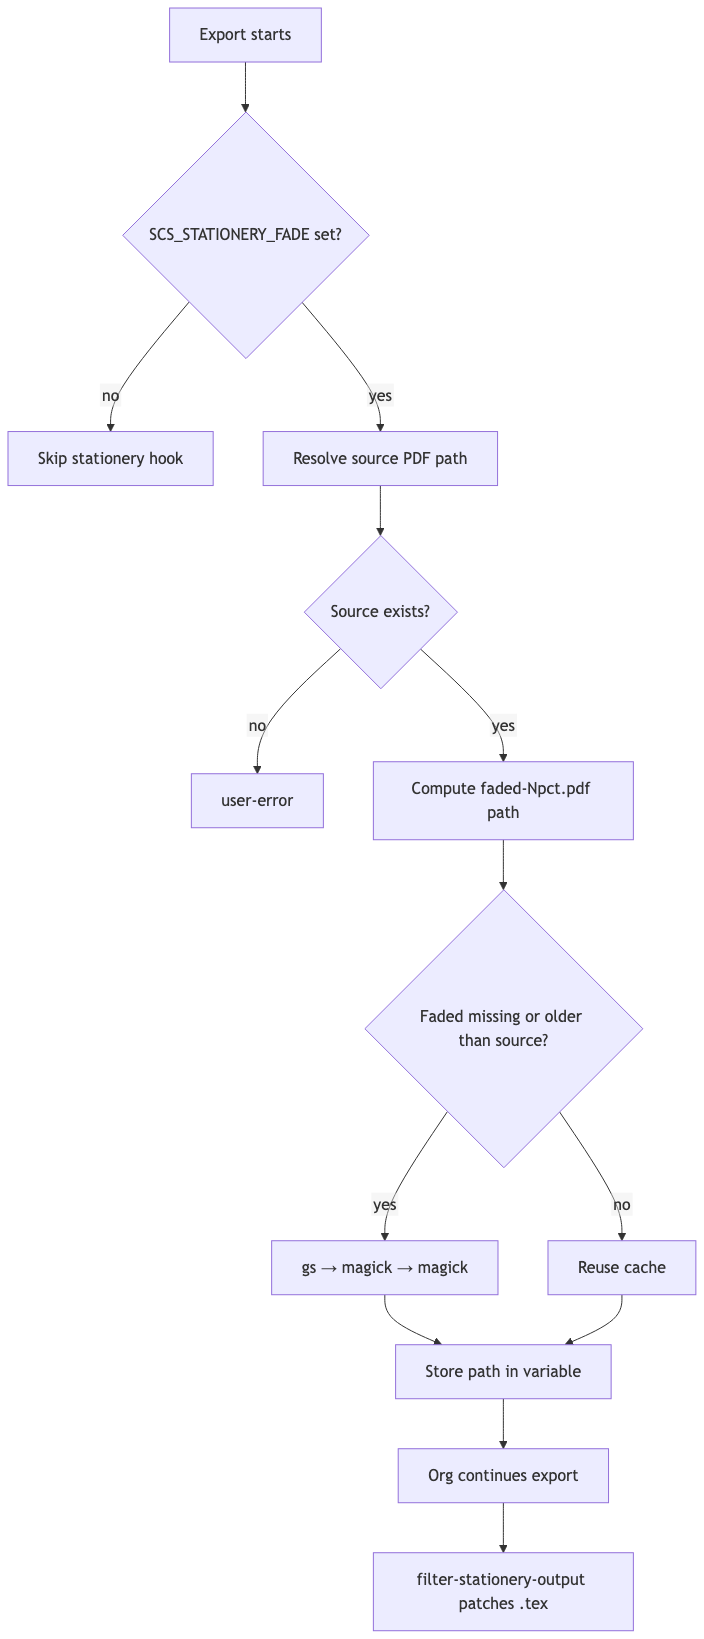
\includegraphics[width=.9\linewidth]{stationery-regenerate.png}
\label{orgc98c080}
\end{center}

\textbf{\textbf{Manual equivalent}} (what the Elisp shim runs):

\begin{verbatim}
SRC=/Users/scs/Documents/scs-stationary.pdf
OUT=/Users/scs/Documents/scs-stationary-faded-27pct.pdf
FADE=27
COLORIZE=$((100 - FADE))   # 73

gs -q -dNOPAUSE -dBATCH -dNOSAFER \
   -sDEVICE=png16m -r300 \
   -sOutputFile=/tmp/page-%03d.png "$SRC"

magick /tmp/page-001.png -background white -alpha remove \
   -fill white -colorize ${COLORIZE}% /tmp/faded.png

magick /tmp/faded.png -units PixelsPerInch -density 300 \
   -compress zip "$OUT"
\end{verbatim}

\textbf{\textbf{Placeholder substitution}} happens on the \textbf{final \LaTeX{} string}, not in the
export buffer (Org assembles \texttt{\#+LATEX\_HEADER} separately).  Substitution uses
\texttt{replace-match} with \texttt{fixedcase} so paths like \texttt{/Users/scs/...} are not
corrupted (plain \texttt{replace-regexp-in-string} uppercased paths because of
\texttt{\textbackslash{}U} escape rules in replacement templates).
\section*{Example packing-list.org skeleton}
\label{sec:org11a4c1e}

\begin{verbatim}
#+TITLE: Packing checklist
#+SCS_STATIONERY: /Users/scs/Documents/scs-stationary.pdf
#+SCS_STATIONERY_FADE: 27
#+LATEX_COMPILER: lualatex

#+LATEX_HEADER: \usepackage{eso-pic}
#+LATEX_HEADER: \usepackage{geometry}
#+LATEX_HEADER: \geometry{...}
#+LATEX_HEADER: \AddToShipoutPictureBG{...{SCS_STATIONERY_FADED_PDF}}}
#+LATEX_HEADER: \usepackage{microtype}
#+LATEX_HEADER: \input{/Users/scs/fonts/scs-canon/scs-fontspec.tex}
#+LATEX_HEADER: \fancyhead[C]{\runheadertext{[packing checklist]}}

... body ...

#+begin_export latex
\vfill \vspace{-0.5em}
#+end_export

!sc footnotesize typeset at tapoban on 4 july 63 sc -- sri chinmoy society press
!sc footnotesize [letterhead colours dimmed on purpose]
\end{verbatim}
\section*{Requirements and troubleshooting}
\label{sec:org13f2b77}

\textbf{\textbf{Requirements}}

\begin{itemize}
\item Emacs ≥ 29.1, Org ≥ 9.0
\item LuaLaTeX (\texttt{\#+LATEX\_COMPILER: lualatex})
\item \texttt{fontspec}, \texttt{eso-pic}, \texttt{fancyhdr}, \texttt{microtype} (via \TeX{} Live)
\item \texttt{gs} (Ghostscript) and \texttt{magick} (ImageMagick) on \texttt{PATH} for stationery fade
\item Fonts in \texttt{/Users/scs/fonts/scs-canon/}
\end{itemize}

\textbf{\textbf{Common issues}}

\begin{center}
\begin{tabular}{lll}
Symptom & Likely cause & What to do\\
\hline
\texttt{!} lines not expanded & \texttt{org-tools} not loaded & \texttt{(require 'org-tools)} in init\\
No small caps & Old \texttt{scs-fontspec.tex} & Reload; check \texttt{Letters=SmallCaps}\\
Line with \texttt{[} missing & fontspec ate \texttt{[} as options & Ensure \texttt{\{\#1\}} wrapper in \texttt{scs-fontspec.tex}\\
\texttt{-{}-{}} not an en-dash in \texttt{!sc} & Missing \texttt{Ligatures=TeX} & Update \texttt{scs-fontspec.tex}\\
Header brackets missing & Fragile \texttt{\textbackslash{}textsc} in \texttt{\textbackslash{}fancyhead} & Use \texttt{\textbackslash{}runheadertext\{...\}}\\
Wrong stationery in PDF & Stale cache & Touch source PDF or \texttt{M-x org-tools-regenerate-stationery}\\
Export error “gs not found” & Ghostscript missing & Install Ghostscript\\
Path all UPPERCASE in \texttt{.tex} & Old substitution bug & Update \texttt{org-tools.el} (use \texttt{replace-match})\\
\end{tabular}
\end{center}

\textbf{\textbf{Useful commands}}

\begin{center}
\begin{tabular}{ll}
Command & Action\\
\hline
\texttt{C-c C-e l l} & Export to \LaTeX{} file\\
\texttt{C-c C-e l p} & Export to PDF (export + compile)\\
\texttt{M-x org-tools-line-prefixes-status} & Check \texttt{!} / => hook\\
\texttt{M-x org-tools-regenerate-stationery} & Rebuild faded letterhead from buffer keywords\\
\end{tabular}
\end{center}
\section*{File index}
\label{sec:orgfede262}

\begin{center}
\begin{tabular}{ll}
Path & Description\\
\hline
\texttt{\textasciitilde{}/.config/emacs/lisp/org-tools.el} & Line prefixes + stationery hooks\\
\texttt{\textasciitilde{}/.config/emacs/lisp/doc/latex-export-hook-explained.org} & This document\\
\texttt{/Users/scs/fonts/scs-canon/scs-fontspec.tex} & Canon font setup\\
\texttt{/Users/scs/fonts/scs-canon/*.otf} & Simoncini + Adobe Garamond files\\
\texttt{\textasciitilde{}/Documents/scs-stationary.pdf} & Full-strength letterhead source\\
\texttt{\textasciitilde{}/Documents/scs-stationary-faded-Npct.pdf} & Cached faded letterhead\\
\end{tabular}
\end{center}
\section*{Viewing Mermaid diagrams in Org}
\label{sec:org1e1836d}

This file uses \texttt{\#+begin\_src mermaid} blocks.  They render when you evaluate
them (\texttt{C-c C-c} on the block) or export the document.

\textbf{\textbf{Setup}} (already in \texttt{init.el}):

\begin{itemize}
\item \texttt{ob-mermaid} (el-get) + \texttt{mermaid} in \texttt{org-babel-load-languages}
\item \texttt{mmdc} from \texttt{npm install -g @mermaid-js/mermaid-cli}
\item Config: \texttt{\textasciitilde{}/.config/mermaid/config.json} (\texttt{htmlLabels: false} for Emacs SVG)
\end{itemize}

\textbf{\textbf{Commands}}

\begin{center}
\begin{tabular}{ll}
Action & Keys\\
\hline
Render one block & \texttt{C-c C-c} on the block\\
Export whole doc & \texttt{C-c C-e h o} (HTML) or \texttt{C-c C-e l p} (PDF via \LaTeX{})\\
\end{tabular}
\end{center}

Diagram PNGs are written beside this file (\texttt{export-pipeline.png},
\texttt{stationery-regenerate.png}).
\section*{History / design notes}
\label{sec:org3a32855}

\begin{itemize}
\item \textbf{scrartcl} was avoided for title placement — Org batch export did not register
the class without extra Elisp; \texttt{titling} + custom \texttt{\textbackslash{}maketitle} on \texttt{article}
was used instead.
\item \textbf{TikZ opacity} on vector stationery worked but was dropped in favour of
pre-faded assets for predictable print output.
\item \textbf{SmallCapsFont=} in a single \texttt{\textbackslash{}setmainfont} block works when all faces share
one directory (\texttt{scs-canon}); cross-directory nested \texttt{SmallCapsFont}{[}Path=\ldots{}]=
failed on \TeX{} Live 2026 fontspec.
\item Stationery placeholder moved from \texttt{@@...@@} to \texttt{SCS\_STATIONERY\_FADED\_PDF}
because Org interprets double-@ as export snippets.
\end{itemize}
\end{document}
